\documentclass[11pt]{article}

    \usepackage[breakable]{tcolorbox}
    \usepackage{parskip} % Stop auto-indenting (to mimic markdown behaviour)
    
    \usepackage{iftex}
    \ifPDFTeX
    	\usepackage[T1]{fontenc}
    	\usepackage{mathpazo}
    \else
    	\usepackage{fontspec}
    \fi

    % Basic figure setup, for now with no caption control since it's done
    % automatically by Pandoc (which extracts ![](path) syntax from Markdown).
    \usepackage{graphicx}
    % Maintain compatibility with old templates. Remove in nbconvert 6.0
    \let\Oldincludegraphics\includegraphics
    % Ensure that by default, figures have no caption (until we provide a
    % proper Figure object with a Caption API and a way to capture that
    % in the conversion process - todo).
    \usepackage{caption}
    \DeclareCaptionFormat{nocaption}{}
    \captionsetup{format=nocaption,aboveskip=0pt,belowskip=0pt}

    \usepackage[Export]{adjustbox} % Used to constrain images to a maximum size
    \adjustboxset{max size={0.9\linewidth}{0.9\paperheight}}
    \usepackage{float}
    \floatplacement{figure}{H} % forces figures to be placed at the correct location
    \usepackage{xcolor} % Allow colors to be defined
    \usepackage{enumerate} % Needed for markdown enumerations to work
    \usepackage{geometry} % Used to adjust the document margins
    \usepackage{amsmath} % Equations
    \usepackage{amssymb} % Equations
    \usepackage{textcomp} % defines textquotesingle
    % Hack from http://tex.stackexchange.com/a/47451/13684:
    \AtBeginDocument{%
        \def\PYZsq{\textquotesingle}% Upright quotes in Pygmentized code
    }
    \usepackage{upquote} % Upright quotes for verbatim code
    \usepackage{eurosym} % defines \euro
    \usepackage[mathletters]{ucs} % Extended unicode (utf-8) support
    \usepackage{fancyvrb} % verbatim replacement that allows latex
    \usepackage{grffile} % extends the file name processing of package graphics 
                         % to support a larger range
    \makeatletter % fix for grffile with XeLaTeX
    \def\Gread@@xetex#1{%
      \IfFileExists{"\Gin@base".bb}%
      {\Gread@eps{\Gin@base.bb}}%
      {\Gread@@xetex@aux#1}%
    }
    \makeatother

    % The hyperref package gives us a pdf with properly built
    % internal navigation ('pdf bookmarks' for the table of contents,
    % internal cross-reference links, web links for URLs, etc.)
    \usepackage{hyperref}
    % The default LaTeX title has an obnoxious amount of whitespace. By default,
    % titling removes some of it. It also provides customization options.
    \usepackage{titling}
    \usepackage{longtable} % longtable support required by pandoc >1.10
    \usepackage{booktabs}  % table support for pandoc > 1.12.2
    \usepackage[inline]{enumitem} % IRkernel/repr support (it uses the enumerate* environment)
    \usepackage[normalem]{ulem} % ulem is needed to support strikethroughs (\sout)
                                % normalem makes italics be italics, not underlines
    \usepackage{mathrsfs}
    

    
    % Colors for the hyperref package
    \definecolor{urlcolor}{rgb}{0,.145,.698}
    \definecolor{linkcolor}{rgb}{.71,0.21,0.01}
    \definecolor{citecolor}{rgb}{.12,.54,.11}

    % ANSI colors
    \definecolor{ansi-black}{HTML}{3E424D}
    \definecolor{ansi-black-intense}{HTML}{282C36}
    \definecolor{ansi-red}{HTML}{E75C58}
    \definecolor{ansi-red-intense}{HTML}{B22B31}
    \definecolor{ansi-green}{HTML}{00A250}
    \definecolor{ansi-green-intense}{HTML}{007427}
    \definecolor{ansi-yellow}{HTML}{DDB62B}
    \definecolor{ansi-yellow-intense}{HTML}{B27D12}
    \definecolor{ansi-blue}{HTML}{208FFB}
    \definecolor{ansi-blue-intense}{HTML}{0065CA}
    \definecolor{ansi-magenta}{HTML}{D160C4}
    \definecolor{ansi-magenta-intense}{HTML}{A03196}
    \definecolor{ansi-cyan}{HTML}{60C6C8}
    \definecolor{ansi-cyan-intense}{HTML}{258F8F}
    \definecolor{ansi-white}{HTML}{C5C1B4}
    \definecolor{ansi-white-intense}{HTML}{A1A6B2}
    \definecolor{ansi-default-inverse-fg}{HTML}{FFFFFF}
    \definecolor{ansi-default-inverse-bg}{HTML}{000000}

    % commands and environments needed by pandoc snippets
    % extracted from the output of `pandoc -s`
    \providecommand{\tightlist}{%
      \setlength{\itemsep}{0pt}\setlength{\parskip}{0pt}}
    \DefineVerbatimEnvironment{Highlighting}{Verbatim}{commandchars=\\\{\}}
    % Add ',fontsize=\small' for more characters per line
    \newenvironment{Shaded}{}{}
    \newcommand{\KeywordTok}[1]{\textcolor[rgb]{0.00,0.44,0.13}{\textbf{{#1}}}}
    \newcommand{\DataTypeTok}[1]{\textcolor[rgb]{0.56,0.13,0.00}{{#1}}}
    \newcommand{\DecValTok}[1]{\textcolor[rgb]{0.25,0.63,0.44}{{#1}}}
    \newcommand{\BaseNTok}[1]{\textcolor[rgb]{0.25,0.63,0.44}{{#1}}}
    \newcommand{\FloatTok}[1]{\textcolor[rgb]{0.25,0.63,0.44}{{#1}}}
    \newcommand{\CharTok}[1]{\textcolor[rgb]{0.25,0.44,0.63}{{#1}}}
    \newcommand{\StringTok}[1]{\textcolor[rgb]{0.25,0.44,0.63}{{#1}}}
    \newcommand{\CommentTok}[1]{\textcolor[rgb]{0.38,0.63,0.69}{\textit{{#1}}}}
    \newcommand{\OtherTok}[1]{\textcolor[rgb]{0.00,0.44,0.13}{{#1}}}
    \newcommand{\AlertTok}[1]{\textcolor[rgb]{1.00,0.00,0.00}{\textbf{{#1}}}}
    \newcommand{\FunctionTok}[1]{\textcolor[rgb]{0.02,0.16,0.49}{{#1}}}
    \newcommand{\RegionMarkerTok}[1]{{#1}}
    \newcommand{\ErrorTok}[1]{\textcolor[rgb]{1.00,0.00,0.00}{\textbf{{#1}}}}
    \newcommand{\NormalTok}[1]{{#1}}
    
    % Additional commands for more recent versions of Pandoc
    \newcommand{\ConstantTok}[1]{\textcolor[rgb]{0.53,0.00,0.00}{{#1}}}
    \newcommand{\SpecialCharTok}[1]{\textcolor[rgb]{0.25,0.44,0.63}{{#1}}}
    \newcommand{\VerbatimStringTok}[1]{\textcolor[rgb]{0.25,0.44,0.63}{{#1}}}
    \newcommand{\SpecialStringTok}[1]{\textcolor[rgb]{0.73,0.40,0.53}{{#1}}}
    \newcommand{\ImportTok}[1]{{#1}}
    \newcommand{\DocumentationTok}[1]{\textcolor[rgb]{0.73,0.13,0.13}{\textit{{#1}}}}
    \newcommand{\AnnotationTok}[1]{\textcolor[rgb]{0.38,0.63,0.69}{\textbf{\textit{{#1}}}}}
    \newcommand{\CommentVarTok}[1]{\textcolor[rgb]{0.38,0.63,0.69}{\textbf{\textit{{#1}}}}}
    \newcommand{\VariableTok}[1]{\textcolor[rgb]{0.10,0.09,0.49}{{#1}}}
    \newcommand{\ControlFlowTok}[1]{\textcolor[rgb]{0.00,0.44,0.13}{\textbf{{#1}}}}
    \newcommand{\OperatorTok}[1]{\textcolor[rgb]{0.40,0.40,0.40}{{#1}}}
    \newcommand{\BuiltInTok}[1]{{#1}}
    \newcommand{\ExtensionTok}[1]{{#1}}
    \newcommand{\PreprocessorTok}[1]{\textcolor[rgb]{0.74,0.48,0.00}{{#1}}}
    \newcommand{\AttributeTok}[1]{\textcolor[rgb]{0.49,0.56,0.16}{{#1}}}
    \newcommand{\InformationTok}[1]{\textcolor[rgb]{0.38,0.63,0.69}{\textbf{\textit{{#1}}}}}
    \newcommand{\WarningTok}[1]{\textcolor[rgb]{0.38,0.63,0.69}{\textbf{\textit{{#1}}}}}
    
    
    % Define a nice break command that doesn't care if a line doesn't already
    % exist.
    \def\br{\hspace*{\fill} \\* }
    % Math Jax compatibility definitions
    \def\gt{>}
    \def\lt{<}
    \let\Oldtex\TeX
    \let\Oldlatex\LaTeX
    \renewcommand{\TeX}{\textrm{\Oldtex}}
    \renewcommand{\LaTeX}{\textrm{\Oldlatex}}
    % Document parameters
    % Document title
    \title{Capitulo\_4}
    
    
    
    
    
% Pygments definitions
\makeatletter
\def\PY@reset{\let\PY@it=\relax \let\PY@bf=\relax%
    \let\PY@ul=\relax \let\PY@tc=\relax%
    \let\PY@bc=\relax \let\PY@ff=\relax}
\def\PY@tok#1{\csname PY@tok@#1\endcsname}
\def\PY@toks#1+{\ifx\relax#1\empty\else%
    \PY@tok{#1}\expandafter\PY@toks\fi}
\def\PY@do#1{\PY@bc{\PY@tc{\PY@ul{%
    \PY@it{\PY@bf{\PY@ff{#1}}}}}}}
\def\PY#1#2{\PY@reset\PY@toks#1+\relax+\PY@do{#2}}

\expandafter\def\csname PY@tok@w\endcsname{\def\PY@tc##1{\textcolor[rgb]{0.73,0.73,0.73}{##1}}}
\expandafter\def\csname PY@tok@c\endcsname{\let\PY@it=\textit\def\PY@tc##1{\textcolor[rgb]{0.25,0.50,0.50}{##1}}}
\expandafter\def\csname PY@tok@cp\endcsname{\def\PY@tc##1{\textcolor[rgb]{0.74,0.48,0.00}{##1}}}
\expandafter\def\csname PY@tok@k\endcsname{\let\PY@bf=\textbf\def\PY@tc##1{\textcolor[rgb]{0.00,0.50,0.00}{##1}}}
\expandafter\def\csname PY@tok@kp\endcsname{\def\PY@tc##1{\textcolor[rgb]{0.00,0.50,0.00}{##1}}}
\expandafter\def\csname PY@tok@kt\endcsname{\def\PY@tc##1{\textcolor[rgb]{0.69,0.00,0.25}{##1}}}
\expandafter\def\csname PY@tok@o\endcsname{\def\PY@tc##1{\textcolor[rgb]{0.40,0.40,0.40}{##1}}}
\expandafter\def\csname PY@tok@ow\endcsname{\let\PY@bf=\textbf\def\PY@tc##1{\textcolor[rgb]{0.67,0.13,1.00}{##1}}}
\expandafter\def\csname PY@tok@nb\endcsname{\def\PY@tc##1{\textcolor[rgb]{0.00,0.50,0.00}{##1}}}
\expandafter\def\csname PY@tok@nf\endcsname{\def\PY@tc##1{\textcolor[rgb]{0.00,0.00,1.00}{##1}}}
\expandafter\def\csname PY@tok@nc\endcsname{\let\PY@bf=\textbf\def\PY@tc##1{\textcolor[rgb]{0.00,0.00,1.00}{##1}}}
\expandafter\def\csname PY@tok@nn\endcsname{\let\PY@bf=\textbf\def\PY@tc##1{\textcolor[rgb]{0.00,0.00,1.00}{##1}}}
\expandafter\def\csname PY@tok@ne\endcsname{\let\PY@bf=\textbf\def\PY@tc##1{\textcolor[rgb]{0.82,0.25,0.23}{##1}}}
\expandafter\def\csname PY@tok@nv\endcsname{\def\PY@tc##1{\textcolor[rgb]{0.10,0.09,0.49}{##1}}}
\expandafter\def\csname PY@tok@no\endcsname{\def\PY@tc##1{\textcolor[rgb]{0.53,0.00,0.00}{##1}}}
\expandafter\def\csname PY@tok@nl\endcsname{\def\PY@tc##1{\textcolor[rgb]{0.63,0.63,0.00}{##1}}}
\expandafter\def\csname PY@tok@ni\endcsname{\let\PY@bf=\textbf\def\PY@tc##1{\textcolor[rgb]{0.60,0.60,0.60}{##1}}}
\expandafter\def\csname PY@tok@na\endcsname{\def\PY@tc##1{\textcolor[rgb]{0.49,0.56,0.16}{##1}}}
\expandafter\def\csname PY@tok@nt\endcsname{\let\PY@bf=\textbf\def\PY@tc##1{\textcolor[rgb]{0.00,0.50,0.00}{##1}}}
\expandafter\def\csname PY@tok@nd\endcsname{\def\PY@tc##1{\textcolor[rgb]{0.67,0.13,1.00}{##1}}}
\expandafter\def\csname PY@tok@s\endcsname{\def\PY@tc##1{\textcolor[rgb]{0.73,0.13,0.13}{##1}}}
\expandafter\def\csname PY@tok@sd\endcsname{\let\PY@it=\textit\def\PY@tc##1{\textcolor[rgb]{0.73,0.13,0.13}{##1}}}
\expandafter\def\csname PY@tok@si\endcsname{\let\PY@bf=\textbf\def\PY@tc##1{\textcolor[rgb]{0.73,0.40,0.53}{##1}}}
\expandafter\def\csname PY@tok@se\endcsname{\let\PY@bf=\textbf\def\PY@tc##1{\textcolor[rgb]{0.73,0.40,0.13}{##1}}}
\expandafter\def\csname PY@tok@sr\endcsname{\def\PY@tc##1{\textcolor[rgb]{0.73,0.40,0.53}{##1}}}
\expandafter\def\csname PY@tok@ss\endcsname{\def\PY@tc##1{\textcolor[rgb]{0.10,0.09,0.49}{##1}}}
\expandafter\def\csname PY@tok@sx\endcsname{\def\PY@tc##1{\textcolor[rgb]{0.00,0.50,0.00}{##1}}}
\expandafter\def\csname PY@tok@m\endcsname{\def\PY@tc##1{\textcolor[rgb]{0.40,0.40,0.40}{##1}}}
\expandafter\def\csname PY@tok@gh\endcsname{\let\PY@bf=\textbf\def\PY@tc##1{\textcolor[rgb]{0.00,0.00,0.50}{##1}}}
\expandafter\def\csname PY@tok@gu\endcsname{\let\PY@bf=\textbf\def\PY@tc##1{\textcolor[rgb]{0.50,0.00,0.50}{##1}}}
\expandafter\def\csname PY@tok@gd\endcsname{\def\PY@tc##1{\textcolor[rgb]{0.63,0.00,0.00}{##1}}}
\expandafter\def\csname PY@tok@gi\endcsname{\def\PY@tc##1{\textcolor[rgb]{0.00,0.63,0.00}{##1}}}
\expandafter\def\csname PY@tok@gr\endcsname{\def\PY@tc##1{\textcolor[rgb]{1.00,0.00,0.00}{##1}}}
\expandafter\def\csname PY@tok@ge\endcsname{\let\PY@it=\textit}
\expandafter\def\csname PY@tok@gs\endcsname{\let\PY@bf=\textbf}
\expandafter\def\csname PY@tok@gp\endcsname{\let\PY@bf=\textbf\def\PY@tc##1{\textcolor[rgb]{0.00,0.00,0.50}{##1}}}
\expandafter\def\csname PY@tok@go\endcsname{\def\PY@tc##1{\textcolor[rgb]{0.53,0.53,0.53}{##1}}}
\expandafter\def\csname PY@tok@gt\endcsname{\def\PY@tc##1{\textcolor[rgb]{0.00,0.27,0.87}{##1}}}
\expandafter\def\csname PY@tok@err\endcsname{\def\PY@bc##1{\setlength{\fboxsep}{0pt}\fcolorbox[rgb]{1.00,0.00,0.00}{1,1,1}{\strut ##1}}}
\expandafter\def\csname PY@tok@kc\endcsname{\let\PY@bf=\textbf\def\PY@tc##1{\textcolor[rgb]{0.00,0.50,0.00}{##1}}}
\expandafter\def\csname PY@tok@kd\endcsname{\let\PY@bf=\textbf\def\PY@tc##1{\textcolor[rgb]{0.00,0.50,0.00}{##1}}}
\expandafter\def\csname PY@tok@kn\endcsname{\let\PY@bf=\textbf\def\PY@tc##1{\textcolor[rgb]{0.00,0.50,0.00}{##1}}}
\expandafter\def\csname PY@tok@kr\endcsname{\let\PY@bf=\textbf\def\PY@tc##1{\textcolor[rgb]{0.00,0.50,0.00}{##1}}}
\expandafter\def\csname PY@tok@bp\endcsname{\def\PY@tc##1{\textcolor[rgb]{0.00,0.50,0.00}{##1}}}
\expandafter\def\csname PY@tok@fm\endcsname{\def\PY@tc##1{\textcolor[rgb]{0.00,0.00,1.00}{##1}}}
\expandafter\def\csname PY@tok@vc\endcsname{\def\PY@tc##1{\textcolor[rgb]{0.10,0.09,0.49}{##1}}}
\expandafter\def\csname PY@tok@vg\endcsname{\def\PY@tc##1{\textcolor[rgb]{0.10,0.09,0.49}{##1}}}
\expandafter\def\csname PY@tok@vi\endcsname{\def\PY@tc##1{\textcolor[rgb]{0.10,0.09,0.49}{##1}}}
\expandafter\def\csname PY@tok@vm\endcsname{\def\PY@tc##1{\textcolor[rgb]{0.10,0.09,0.49}{##1}}}
\expandafter\def\csname PY@tok@sa\endcsname{\def\PY@tc##1{\textcolor[rgb]{0.73,0.13,0.13}{##1}}}
\expandafter\def\csname PY@tok@sb\endcsname{\def\PY@tc##1{\textcolor[rgb]{0.73,0.13,0.13}{##1}}}
\expandafter\def\csname PY@tok@sc\endcsname{\def\PY@tc##1{\textcolor[rgb]{0.73,0.13,0.13}{##1}}}
\expandafter\def\csname PY@tok@dl\endcsname{\def\PY@tc##1{\textcolor[rgb]{0.73,0.13,0.13}{##1}}}
\expandafter\def\csname PY@tok@s2\endcsname{\def\PY@tc##1{\textcolor[rgb]{0.73,0.13,0.13}{##1}}}
\expandafter\def\csname PY@tok@sh\endcsname{\def\PY@tc##1{\textcolor[rgb]{0.73,0.13,0.13}{##1}}}
\expandafter\def\csname PY@tok@s1\endcsname{\def\PY@tc##1{\textcolor[rgb]{0.73,0.13,0.13}{##1}}}
\expandafter\def\csname PY@tok@mb\endcsname{\def\PY@tc##1{\textcolor[rgb]{0.40,0.40,0.40}{##1}}}
\expandafter\def\csname PY@tok@mf\endcsname{\def\PY@tc##1{\textcolor[rgb]{0.40,0.40,0.40}{##1}}}
\expandafter\def\csname PY@tok@mh\endcsname{\def\PY@tc##1{\textcolor[rgb]{0.40,0.40,0.40}{##1}}}
\expandafter\def\csname PY@tok@mi\endcsname{\def\PY@tc##1{\textcolor[rgb]{0.40,0.40,0.40}{##1}}}
\expandafter\def\csname PY@tok@il\endcsname{\def\PY@tc##1{\textcolor[rgb]{0.40,0.40,0.40}{##1}}}
\expandafter\def\csname PY@tok@mo\endcsname{\def\PY@tc##1{\textcolor[rgb]{0.40,0.40,0.40}{##1}}}
\expandafter\def\csname PY@tok@ch\endcsname{\let\PY@it=\textit\def\PY@tc##1{\textcolor[rgb]{0.25,0.50,0.50}{##1}}}
\expandafter\def\csname PY@tok@cm\endcsname{\let\PY@it=\textit\def\PY@tc##1{\textcolor[rgb]{0.25,0.50,0.50}{##1}}}
\expandafter\def\csname PY@tok@cpf\endcsname{\let\PY@it=\textit\def\PY@tc##1{\textcolor[rgb]{0.25,0.50,0.50}{##1}}}
\expandafter\def\csname PY@tok@c1\endcsname{\let\PY@it=\textit\def\PY@tc##1{\textcolor[rgb]{0.25,0.50,0.50}{##1}}}
\expandafter\def\csname PY@tok@cs\endcsname{\let\PY@it=\textit\def\PY@tc##1{\textcolor[rgb]{0.25,0.50,0.50}{##1}}}

\def\PYZbs{\char`\\}
\def\PYZus{\char`\_}
\def\PYZob{\char`\{}
\def\PYZcb{\char`\}}
\def\PYZca{\char`\^}
\def\PYZam{\char`\&}
\def\PYZlt{\char`\<}
\def\PYZgt{\char`\>}
\def\PYZsh{\char`\#}
\def\PYZpc{\char`\%}
\def\PYZdl{\char`\$}
\def\PYZhy{\char`\-}
\def\PYZsq{\char`\'}
\def\PYZdq{\char`\"}
\def\PYZti{\char`\~}
% for compatibility with earlier versions
\def\PYZat{@}
\def\PYZlb{[}
\def\PYZrb{]}
\makeatother


    % For linebreaks inside Verbatim environment from package fancyvrb. 
    \makeatletter
        \newbox\Wrappedcontinuationbox 
        \newbox\Wrappedvisiblespacebox 
        \newcommand*\Wrappedvisiblespace {\textcolor{red}{\textvisiblespace}} 
        \newcommand*\Wrappedcontinuationsymbol {\textcolor{red}{\llap{\tiny$\m@th\hookrightarrow$}}} 
        \newcommand*\Wrappedcontinuationindent {3ex } 
        \newcommand*\Wrappedafterbreak {\kern\Wrappedcontinuationindent\copy\Wrappedcontinuationbox} 
        % Take advantage of the already applied Pygments mark-up to insert 
        % potential linebreaks for TeX processing. 
        %        {, <, #, %, $, ' and ": go to next line. 
        %        _, }, ^, &, >, - and ~: stay at end of broken line. 
        % Use of \textquotesingle for straight quote. 
        \newcommand*\Wrappedbreaksatspecials {% 
            \def\PYGZus{\discretionary{\char`\_}{\Wrappedafterbreak}{\char`\_}}% 
            \def\PYGZob{\discretionary{}{\Wrappedafterbreak\char`\{}{\char`\{}}% 
            \def\PYGZcb{\discretionary{\char`\}}{\Wrappedafterbreak}{\char`\}}}% 
            \def\PYGZca{\discretionary{\char`\^}{\Wrappedafterbreak}{\char`\^}}% 
            \def\PYGZam{\discretionary{\char`\&}{\Wrappedafterbreak}{\char`\&}}% 
            \def\PYGZlt{\discretionary{}{\Wrappedafterbreak\char`\<}{\char`\<}}% 
            \def\PYGZgt{\discretionary{\char`\>}{\Wrappedafterbreak}{\char`\>}}% 
            \def\PYGZsh{\discretionary{}{\Wrappedafterbreak\char`\#}{\char`\#}}% 
            \def\PYGZpc{\discretionary{}{\Wrappedafterbreak\char`\%}{\char`\%}}% 
            \def\PYGZdl{\discretionary{}{\Wrappedafterbreak\char`\$}{\char`\$}}% 
            \def\PYGZhy{\discretionary{\char`\-}{\Wrappedafterbreak}{\char`\-}}% 
            \def\PYGZsq{\discretionary{}{\Wrappedafterbreak\textquotesingle}{\textquotesingle}}% 
            \def\PYGZdq{\discretionary{}{\Wrappedafterbreak\char`\"}{\char`\"}}% 
            \def\PYGZti{\discretionary{\char`\~}{\Wrappedafterbreak}{\char`\~}}% 
        } 
        % Some characters . , ; ? ! / are not pygmentized. 
        % This macro makes them "active" and they will insert potential linebreaks 
        \newcommand*\Wrappedbreaksatpunct {% 
            \lccode`\~`\.\lowercase{\def~}{\discretionary{\hbox{\char`\.}}{\Wrappedafterbreak}{\hbox{\char`\.}}}% 
            \lccode`\~`\,\lowercase{\def~}{\discretionary{\hbox{\char`\,}}{\Wrappedafterbreak}{\hbox{\char`\,}}}% 
            \lccode`\~`\;\lowercase{\def~}{\discretionary{\hbox{\char`\;}}{\Wrappedafterbreak}{\hbox{\char`\;}}}% 
            \lccode`\~`\:\lowercase{\def~}{\discretionary{\hbox{\char`\:}}{\Wrappedafterbreak}{\hbox{\char`\:}}}% 
            \lccode`\~`\?\lowercase{\def~}{\discretionary{\hbox{\char`\?}}{\Wrappedafterbreak}{\hbox{\char`\?}}}% 
            \lccode`\~`\!\lowercase{\def~}{\discretionary{\hbox{\char`\!}}{\Wrappedafterbreak}{\hbox{\char`\!}}}% 
            \lccode`\~`\/\lowercase{\def~}{\discretionary{\hbox{\char`\/}}{\Wrappedafterbreak}{\hbox{\char`\/}}}% 
            \catcode`\.\active
            \catcode`\,\active 
            \catcode`\;\active
            \catcode`\:\active
            \catcode`\?\active
            \catcode`\!\active
            \catcode`\/\active 
            \lccode`\~`\~ 	
        }
    \makeatother

    \let\OriginalVerbatim=\Verbatim
    \makeatletter
    \renewcommand{\Verbatim}[1][1]{%
        %\parskip\z@skip
        \sbox\Wrappedcontinuationbox {\Wrappedcontinuationsymbol}%
        \sbox\Wrappedvisiblespacebox {\FV@SetupFont\Wrappedvisiblespace}%
        \def\FancyVerbFormatLine ##1{\hsize\linewidth
            \vtop{\raggedright\hyphenpenalty\z@\exhyphenpenalty\z@
                \doublehyphendemerits\z@\finalhyphendemerits\z@
                \strut ##1\strut}%
        }%
        % If the linebreak is at a space, the latter will be displayed as visible
        % space at end of first line, and a continuation symbol starts next line.
        % Stretch/shrink are however usually zero for typewriter font.
        \def\FV@Space {%
            \nobreak\hskip\z@ plus\fontdimen3\font minus\fontdimen4\font
            \discretionary{\copy\Wrappedvisiblespacebox}{\Wrappedafterbreak}
            {\kern\fontdimen2\font}%
        }%
        
        % Allow breaks at special characters using \PYG... macros.
        \Wrappedbreaksatspecials
        % Breaks at punctuation characters . , ; ? ! and / need catcode=\active 	
        \OriginalVerbatim[#1,codes*=\Wrappedbreaksatpunct]%
    }
    \makeatother

    % Exact colors from NB
    \definecolor{incolor}{HTML}{303F9F}
    \definecolor{outcolor}{HTML}{D84315}
    \definecolor{cellborder}{HTML}{CFCFCF}
    \definecolor{cellbackground}{HTML}{F7F7F7}
    
    % prompt
    \makeatletter
    \newcommand{\boxspacing}{\kern\kvtcb@left@rule\kern\kvtcb@boxsep}
    \makeatother
    \newcommand{\prompt}[4]{
        \ttfamily\llap{{\color{#2}[#3]:\hspace{3pt}#4}}\vspace{-\baselineskip}
    }
    

    
    % Prevent overflowing lines due to hard-to-break entities
    \sloppy 
    % Setup hyperref package
    \hypersetup{
      breaklinks=true,  % so long urls are correctly broken across lines
      colorlinks=true,
      urlcolor=urlcolor,
      linkcolor=linkcolor,
      citecolor=citecolor,
      }
    % Slightly bigger margins than the latex defaults
    
    \geometry{verbose,tmargin=1in,bmargin=1in,lmargin=1in,rmargin=1in}
    
    

\begin{document}
    
    \maketitle
    
    

    
    \hypertarget{capuxedtulo-4-multiplexaciuxf3n-en-frecuencia-fdm-frequency-division-multiplexing}{%
\section{Capítulo 4: MULTIPLEXACIÓN EN FRECUENCIA, FDM (FREQUENCY
DIVISION
MULTIPLEXING)}\label{capuxedtulo-4-multiplexaciuxf3n-en-frecuencia-fdm-frequency-division-multiplexing}}

    \hypertarget{evaluaciuxf3n}{%
\subsection{Evaluación}\label{evaluaciuxf3n}}

\hypertarget{defina}{%
\subsubsection{Defina:}\label{defina}}

\begin{itemize}
\tightlist
\item
  \textbf{Interferencia Inter-Canal} : La interferencia inter-canal se
  produce cuando los componentes espectrales de canales adyacentes se
  mezclan uno con el otro, produciendo distorción en las señales. Este
  fenomeno se puede presentar cuando no se realiza un adecuado filtrado,
  o no se sintoniza bien el canal. Una forma de solucionarlo ha sido la
  implementación de las llamadas bandas de guarda, que son una
  separación de los canales en el espectro.
\end{itemize}

\includegraphics{./images/banda_guarda.png}

\begin{itemize}
\tightlist
\item
  \textbf{Multiplexación en el dominio de la frecuencia} : Como se sabe
  el concepto básico de multiplexar es usar un mismo canal para varios
  usuarios a la vez, entonces como en la multiplexación en el tiempo
  donde a cada usuario le damos un espacio de tiempo para transmitir, en
  la frecuencia le damos al usuario un rango de frecuencias que debe
  estar dentro del las frecuencias admisibles por medio de transmición,
  en la siguiente imagen se ilustra este concepto
\end{itemize}

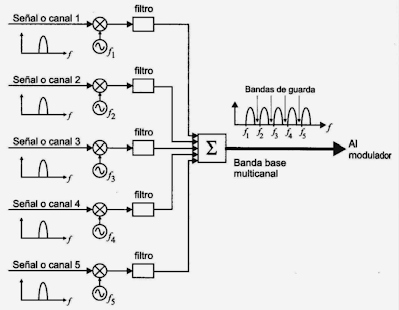
\includegraphics{./images/FDM.png}

\begin{itemize}
\tightlist
\item
  \textbf{Esquema de transmisión Gridless}: Este esquema se basa en que
  todos los canales no necitan igual ancho de banda todo el tiempo, en
  otras palabras tiene en cuenta la dinámica de cada canal al requerir
  ancho de banda, con ello en mente no tiene rangos de frecuencia fijos
  para cada canal, si no que van mutando, incrementado o decrementando,
  según el canal lo requiera. En la siguiente imagen se puede ver una
  comparación de Fized Grid y GridLess en fibra optica.
\end{itemize}

\includegraphics{./images/gridless.jpg}

    \hypertarget{simulaciones}{%
\subsubsection{Simulaciones}\label{simulaciones}}

\includegraphics{./images/ejercicio.png}

\begin{itemize}
\tightlist
\item
  \textbf{Implemente la solución del ejercicio de diseño propuesto en la
  diapositiva 63}
\item
  \textbf{Estime la relación entre ICI (expresado en HZ) y tasa de
  error}
\end{itemize}

\hypertarget{capacidad-del-canal}{%
\paragraph{Capacidad del Canal}\label{capacidad-del-canal}}

La capacidad de un canal la podemos medir de la siguiente forma Según
Nyquist:

\[C = 2B\log_2{N}\ \ [bps]\]

Según Shannon:

\[C = B\log_2(1 + SNR)\ \ [bps]\]

donde \(B\) es el nacho de banda analogico, \(N\) es el numéro de
simbolos del esquema de modulación y \(SNR\) es la relación señal a
ruido.

Para el ejercicio vamos a utilizar un valore de \(SNR_{dB} = 25 \ dB\)
lo que sería igual a \(SNR = 316.22\)

Con lo que tendriamos aproximadamente

\[C = 8B \ \ [bps]\]

    \hypertarget{soluciuxf3n-del-problema-de-diseuxf1o}{%
\paragraph{Solución del problema de
diseño}\label{soluciuxf3n-del-problema-de-diseuxf1o}}

\begin{itemize}
\item
  \textbf{Canal 1}: Roll-Off = 1.0, Baudio : 15 MBaud

  \begin{itemize}
  \item
    Qué formato de modulación se esta usando?

    Para aproximarnos al formato de modulación necesitamo primero saber
    cuanto es la capacidad del canal \[C = (8)(30)10^6 = 240Mbps \] El
    numéro de simbolos \[N = 2^{\frac{C}{2B}} =16\]

    Como se puede ver la modulación debe tener 16 simbolos, aqui se
    plantea la modulación 16 QAM
  \item
    Cuál es el valor de \(w_1\)?

    El valor de \(w_1 = 10MHz + \frac{30MHz}{2} = 25MHz\)
  \end{itemize}
\item
  \textbf{Canal 2}: Roll-Off = 1.0, Baudio: 20 MBaud

  \begin{itemize}
  \item
    Qué banda ocupa?

    Ancho de banda = \(2 * 20*10^6 = 40MHz\)

    La banda seria de \(10MHz + 30MHz + 1MHz = 41MHz\) hasta
    \(41MHz+40MHz = 81 MHz\)
  \item
    Cual es el valor de \(w_2\)?
  \end{itemize}

  El valor de \(w_2 = 41MHz + \frac{81MHz - 41MHz}{2} = 61MHz\)
\item
  \textbf{Canal 3}:

  \begin{itemize}
  \tightlist
  \item
    Qué formato de modulación se esta usando?
  \end{itemize}

  Capacidad del canal \[C = (8)(20)10^6 = 160Mbps\] El numéro de
  simbolos \[N = 2^{\frac{C}{2B}} = 4\]

\begin{verbatim}
Se podira usar 4-PSK 
\end{verbatim}

  \begin{itemize}
  \item
    Cuál es el valor de \(w_3\)?

    El valor de \(w_2 = 81MHz+ 1MHz + \frac{20MHz}{2} = 92MHz\)
  \end{itemize}
\item
  \textbf{Canal 4}:Roll-Off = 0.5 Qué formato de modulación debemos
  implementar para completar una tasa de transmisión de 195 Mbaud en los
  100 MHz de los cuatro canales?

  Con un Roll-off = 0.5 se y 195 Mbaud se necesitaria 292.5 MHz, no es
  posible a gragarlo en el espaciamiento de 100MHz
\end{itemize}

\textbf{Simulaciones} Por dificultades en la simulación con esas
frecuencias voy a mapear las frecuencias \(1M\) a \(1\)

    \begin{tcolorbox}[breakable, size=fbox, boxrule=1pt, pad at break*=1mm,colback=cellbackground, colframe=cellborder]
\prompt{In}{incolor}{135}{\boxspacing}
\begin{Verbatim}[commandchars=\\\{\}]
\PY{k+kn}{import} \PY{n+nn}{numpy} \PY{k}{as} \PY{n+nn}{np} 
\PY{k+kn}{import} \PY{n+nn}{matplotlib}\PY{n+nn}{.}\PY{n+nn}{pyplot} \PY{k}{as} \PY{n+nn}{plt} 
\PY{k+kn}{import} \PY{n+nn}{komm}

\PY{n}{fs} \PY{o}{=} \PY{l+m+mi}{10000} \PY{c+c1}{\PYZsh{}frecuencia \PYZdq{}real\PYZdq{} de muestreo }
\end{Verbatim}
\end{tcolorbox}

    \begin{tcolorbox}[breakable, size=fbox, boxrule=1pt, pad at break*=1mm,colback=cellbackground, colframe=cellborder]
\prompt{In}{incolor}{236}{\boxspacing}
\begin{Verbatim}[commandchars=\\\{\}]
\PY{k}{def} \PY{n+nf}{x\PYZus{}t}\PY{p}{(}\PY{n}{simbols}\PY{p}{,}\PY{n}{tS}\PY{p}{,}\PY{n}{fc}\PY{o}{=}\PY{l+m+mi}{1}\PY{p}{,}\PY{n}{separadas}\PY{o}{=}\PY{k+kc}{False}\PY{p}{)}\PY{p}{:}
    \PY{l+s+sd}{\PYZdq{}\PYZdq{}\PYZdq{}tS timepo de duración del simbolo\PYZdq{}\PYZdq{}\PYZdq{}}
    \PY{n}{t\PYZus{}c} \PY{o}{=} \PY{n}{np}\PY{o}{.}\PY{n}{arange}\PY{p}{(}\PY{l+m+mi}{0}\PY{p}{,}\PY{n}{tS}\PY{p}{,}\PY{l+m+mi}{1}\PY{o}{/}\PY{n}{fs}\PY{p}{)}
    
    \PY{n}{tf} \PY{o}{=} \PY{n}{tS}\PY{o}{*}\PY{n+nb}{len}\PY{p}{(}\PY{n}{simbols}\PY{p}{)}
    \PY{n}{t} \PY{o}{=} \PY{n}{np}\PY{o}{.}\PY{n}{arange}\PY{p}{(}\PY{l+m+mi}{0}\PY{p}{,}\PY{n}{tf}\PY{p}{,}\PY{l+m+mi}{1}\PY{o}{/}\PY{n}{fs}\PY{p}{)}

    \PY{n}{x} \PY{o}{=} \PY{n}{np}\PY{o}{.}\PY{n}{cos}\PY{p}{(}\PY{l+m+mi}{2}\PY{o}{*}\PY{n}{np}\PY{o}{.}\PY{n}{pi}\PY{o}{*}\PY{n}{t\PYZus{}c}\PY{o}{*}\PY{n}{fc}\PY{p}{)}
    \PY{n}{y} \PY{o}{=} \PY{n}{np}\PY{o}{.}\PY{n}{sin}\PY{p}{(}\PY{l+m+mi}{2}\PY{o}{*}\PY{n}{np}\PY{o}{.}\PY{n}{pi}\PY{o}{*}\PY{n}{t\PYZus{}c}\PY{o}{*}\PY{n}{fc}\PY{p}{)}
    
    \PY{k}{if} \PY{o+ow}{not} \PY{n}{separadas}\PY{p}{:}
        \PY{n}{fm} \PY{o}{=} \PY{n}{np}\PY{o}{.}\PY{n}{array}\PY{p}{(}\PY{p}{[}\PY{p}{]}\PY{p}{)}
        \PY{k}{for} \PY{n}{i} \PY{o+ow}{in} \PY{n}{simbols}\PY{p}{:}
            \PY{n}{fm} \PY{o}{=} \PY{n}{np}\PY{o}{.}\PY{n}{append}\PY{p}{(}\PY{n}{fm}\PY{p}{,} \PY{n}{i}\PY{o}{.}\PY{n}{real}\PY{o}{*}\PY{n}{x}\PY{o}{\PYZhy{}}\PY{n}{i}\PY{o}{.}\PY{n}{imag}\PY{o}{*}\PY{n}{y}\PY{p}{)} 
        \PY{k}{return} \PY{n}{t}\PY{p}{,}\PY{n}{fm}\PY{p}{[}\PY{p}{:}\PY{n+nb}{len}\PY{p}{(}\PY{n}{t}\PY{p}{)}\PY{p}{]}
    
    \PY{k}{else}\PY{p}{:} 
        \PY{n}{phase} \PY{o}{=} \PY{n}{np}\PY{o}{.}\PY{n}{array}\PY{p}{(}\PY{p}{[}\PY{p}{]}\PY{p}{)}
        \PY{n}{qua} \PY{o}{=} \PY{n}{np}\PY{o}{.}\PY{n}{array}\PY{p}{(}\PY{p}{[}\PY{p}{]}\PY{p}{)}
        \PY{k}{for} \PY{n}{i} \PY{o+ow}{in} \PY{n}{simbols}\PY{p}{:}
            \PY{n}{phase} \PY{o}{=} \PY{n}{np}\PY{o}{.}\PY{n}{append}\PY{p}{(}\PY{n}{phase}\PY{p}{,} \PY{n}{i}\PY{o}{.}\PY{n}{real}\PY{o}{*}\PY{n}{x}\PY{p}{)} 
            \PY{n}{qua} \PY{o}{=} \PY{n}{np}\PY{o}{.}\PY{n}{append}\PY{p}{(}\PY{n}{qua}\PY{p}{,}\PY{n}{i}\PY{o}{.}\PY{n}{imag}\PY{o}{*}\PY{n}{y}\PY{p}{)} 
        \PY{k}{return} \PY{n}{phase}\PY{p}{,}\PY{n}{qua}
    
    
\PY{k}{def} \PY{n+nf}{raisedCosinePulse}\PY{p}{(}\PY{n}{t}\PY{p}{,}\PY{n}{roll\PYZus{}off}\PY{o}{=}\PY{l+m+mf}{0.0}\PY{p}{,}\PY{n}{span}\PY{o}{=}\PY{l+m+mi}{1}\PY{p}{)}\PY{p}{:}
    \PY{k}{return} \PY{n}{np}\PY{o}{.}\PY{n}{sinc}\PY{p}{(}\PY{n}{t}\PY{o}{/}\PY{n}{span}\PY{p}{)}\PY{o}{*}\PY{n}{np}\PY{o}{.}\PY{n}{cos}\PY{p}{(}\PY{n}{np}\PY{o}{.}\PY{n}{pi}\PY{o}{*}\PY{n}{roll\PYZus{}off}\PY{o}{*}\PY{n}{t}\PY{o}{/}\PY{n}{span}\PY{p}{)}\PY{o}{/}\PY{p}{(}\PY{l+m+mi}{1}\PY{o}{\PYZhy{}}\PY{p}{(}\PY{l+m+mi}{4}\PY{o}{*}\PY{n}{roll\PYZus{}off}\PY{o}{*}\PY{o}{*}\PY{l+m+mi}{2}\PY{o}{*}\PY{n}{t}\PY{o}{*}\PY{o}{*}\PY{l+m+mi}{2}\PY{p}{)}\PY{o}{/}\PY{n}{span}\PY{o}{*}\PY{o}{*}\PY{l+m+mi}{2}\PY{p}{)}

\PY{k}{def} \PY{n+nf}{rootRaisedCosinePulse}\PY{p}{(}\PY{n}{t}\PY{p}{,}\PY{n}{roll\PYZus{}off}\PY{o}{=}\PY{l+m+mi}{1}\PY{p}{,}\PY{n}{span}\PY{o}{=}\PY{l+m+mi}{1}\PY{p}{)}\PY{p}{:}
    \PY{n}{a} \PY{o}{=} \PY{p}{(}\PY{l+m+mi}{2}\PY{o}{*}\PY{n}{roll\PYZus{}off}\PY{p}{)}\PY{o}{/}\PY{p}{(}\PY{n}{np}\PY{o}{.}\PY{n}{pi}\PY{o}{*}\PY{n}{np}\PY{o}{.}\PY{n}{sqrt}\PY{p}{(}\PY{n}{span}\PY{p}{)}\PY{p}{)}
    \PY{n}{b} \PY{o}{=} \PY{p}{(}\PY{n}{np}\PY{o}{.}\PY{n}{cos}\PY{p}{(}\PY{p}{(}\PY{l+m+mi}{1}\PY{o}{+}\PY{n}{roll\PYZus{}off}\PY{p}{)}\PY{o}{*}\PY{n}{np}\PY{o}{.}\PY{n}{pi}\PY{o}{*}\PY{n}{t}\PY{o}{/}\PY{n}{span}\PY{p}{)}\PY{o}{+} \PY{n}{np}\PY{o}{.}\PY{n}{sin}\PY{p}{(}\PY{p}{(}\PY{l+m+mi}{1}\PY{o}{\PYZhy{}}\PY{n}{roll\PYZus{}off}\PY{p}{)}\PY{o}{*}\PY{n}{np}\PY{o}{.}\PY{n}{pi}\PY{o}{*}\PY{n}{t}\PY{o}{/}\PY{n}{span}\PY{p}{)}\PY{o}{/}\PY{p}{(}\PY{l+m+mi}{4}\PY{o}{*}\PY{n}{roll\PYZus{}off}\PY{o}{*}\PY{n}{t}\PY{o}{/}\PY{n}{span} \PY{p}{)}\PY{p}{)}
    \PY{k}{return} \PY{n}{a}\PY{o}{*}\PY{n}{b}\PY{o}{/}\PY{p}{(}\PY{l+m+mi}{1}\PY{o}{\PYZhy{}}\PY{p}{(}\PY{l+m+mi}{4}\PY{o}{*}\PY{n}{roll\PYZus{}off}\PY{o}{*}\PY{n}{t}\PY{o}{/}\PY{n}{span}\PY{p}{)}\PY{o}{*}\PY{o}{*}\PY{l+m+mi}{2}\PY{p}{)}
\end{Verbatim}
\end{tcolorbox}

    \begin{tcolorbox}[breakable, size=fbox, boxrule=1pt, pad at break*=1mm,colback=cellbackground, colframe=cellborder]
\prompt{In}{incolor}{211}{\boxspacing}
\begin{Verbatim}[commandchars=\\\{\}]
\PY{n}{bits} \PY{o}{=} \PY{n}{np}\PY{o}{.}\PY{n}{random}\PY{o}{.}\PY{n}{randint}\PY{p}{(}\PY{l+m+mi}{0}\PY{p}{,}\PY{l+m+mi}{2}\PY{p}{,}\PY{l+m+mi}{256}\PY{p}{)}
\end{Verbatim}
\end{tcolorbox}

    \begin{tcolorbox}[breakable, size=fbox, boxrule=1pt, pad at break*=1mm,colback=cellbackground, colframe=cellborder]
\prompt{In}{incolor}{220}{\boxspacing}
\begin{Verbatim}[commandchars=\\\{\}]
\PY{n}{canal\PYZus{}1} \PY{o}{=} \PY{n}{komm}\PY{o}{.}\PY{n}{QAModulation}\PY{p}{(}\PY{l+m+mi}{16}\PY{p}{)}
\PY{n}{simbols} \PY{o}{=} \PY{n}{canal\PYZus{}1}\PY{o}{.}\PY{n}{modulate}\PY{p}{(}\PY{n}{bits}\PY{p}{)}
\PY{n}{C1t\PYZus{}}\PY{p}{,}\PY{n}{C1xt} \PY{o}{=} \PY{n}{x\PYZus{}t}\PY{p}{(}\PY{n}{simbols}\PY{p}{,}\PY{n}{tS}\PY{o}{=}\PY{l+m+mf}{1.}\PY{o}{/}\PY{l+m+mf}{15.}\PY{p}{,}\PY{n}{fc}\PY{o}{=}\PY{l+m+mi}{25}\PY{p}{,}\PY{n}{separadas}\PY{o}{=}\PY{k+kc}{False}\PY{p}{)}

\PY{n}{canal\PYZus{}2} \PY{o}{=} \PY{n}{komm}\PY{o}{.}\PY{n}{QAModulation}\PY{p}{(}\PY{l+m+mi}{16}\PY{p}{)}
\PY{n}{simbols} \PY{o}{=} \PY{n}{canal\PYZus{}2}\PY{o}{.}\PY{n}{modulate}\PY{p}{(}\PY{n}{bits}\PY{p}{)}
\PY{n}{C2t\PYZus{}}\PY{p}{,}\PY{n}{C2xt} \PY{o}{=} \PY{n}{x\PYZus{}t}\PY{p}{(}\PY{n}{simbols}\PY{p}{,}\PY{n}{tS}\PY{o}{=}\PY{l+m+mf}{1.}\PY{o}{/}\PY{l+m+mf}{20.}\PY{p}{,}\PY{n}{fc}\PY{o}{=}\PY{l+m+mi}{61}\PY{p}{,}\PY{n}{separadas}\PY{o}{=}\PY{k+kc}{False}\PY{p}{)}

\PY{n}{canal\PYZus{}3} \PY{o}{=} \PY{n}{komm}\PY{o}{.}\PY{n}{PSKModulation}\PY{p}{(}\PY{l+m+mi}{4}\PY{p}{,}\PY{n}{phase\PYZus{}offset}\PY{o}{=}\PY{n}{np}\PY{o}{.}\PY{n}{pi}\PY{o}{/}\PY{l+m+mi}{4}\PY{p}{)}
\PY{n}{simbols} \PY{o}{=} \PY{n}{canal\PYZus{}3}\PY{o}{.}\PY{n}{modulate}\PY{p}{(}\PY{n}{bits}\PY{p}{)}
\PY{n}{C3t\PYZus{}}\PY{p}{,}\PY{n}{C3xt} \PY{o}{=} \PY{n}{x\PYZus{}t}\PY{p}{(}\PY{n}{simbols}\PY{p}{,}\PY{n}{tS}\PY{o}{=}\PY{l+m+mf}{1.}\PY{o}{/}\PY{l+m+mf}{20.}\PY{p}{,}\PY{n}{fc}\PY{o}{=}\PY{l+m+mi}{92}\PY{p}{,}\PY{n}{separadas}\PY{o}{=}\PY{k+kc}{False}\PY{p}{)}
\PY{n+nb}{len}\PY{p}{(}\PY{n}{C1xt}\PY{p}{)}
\end{Verbatim}
\end{tcolorbox}

            \begin{tcolorbox}[breakable, size=fbox, boxrule=.5pt, pad at break*=1mm, opacityfill=0]
\prompt{Out}{outcolor}{220}{\boxspacing}
\begin{Verbatim}[commandchars=\\\{\}]
42667
\end{Verbatim}
\end{tcolorbox}
        
    \begin{tcolorbox}[breakable, size=fbox, boxrule=1pt, pad at break*=1mm,colback=cellbackground, colframe=cellborder]
\prompt{In}{incolor}{243}{\boxspacing}
\begin{Verbatim}[commandchars=\\\{\}]
\PY{n}{roll\PYZus{}offs} \PY{o}{=} \PY{p}{[}\PY{l+m+mf}{0.99}\PY{p}{,}\PY{l+m+mf}{0.99}\PY{p}{,}\PY{l+m+mf}{0.0001}\PY{p}{]}
\PY{n}{channels} \PY{o}{=} \PY{p}{[}\PY{n}{C1xt}\PY{p}{,}\PY{n}{C2xt}\PY{p}{,}\PY{n}{C3xt}\PY{p}{]}
\PY{n}{f\PYZus{}carriers} \PY{o}{=} \PY{p}{[}\PY{l+m+mi}{25}\PY{p}{,}\PY{l+m+mi}{61}\PY{p}{,}\PY{l+m+mi}{92}\PY{p}{]}
\PY{k}{for} \PY{n}{xt} \PY{o+ow}{in} \PY{n}{channels}\PY{p}{:}
    \PY{n}{F} \PY{o}{=} \PY{n}{np}\PY{o}{.}\PY{n}{fft}\PY{o}{.}\PY{n}{fft}\PY{p}{(}\PY{n}{xt}\PY{p}{)} 
    \PY{n}{f\PYZus{}} \PY{o}{=} \PY{n}{np}\PY{o}{.}\PY{n}{fft}\PY{o}{.}\PY{n}{fftfreq}\PY{p}{(}\PY{n+nb}{len}\PY{p}{(}\PY{n}{F}\PY{p}{)}\PY{p}{,}\PY{l+m+mi}{1}\PY{o}{/}\PY{n}{fs}\PY{p}{)}
    \PY{n}{plt}\PY{o}{.}\PY{n}{plot}\PY{p}{(}\PY{n}{f\PYZus{}}\PY{p}{[}\PY{n+nb}{range}\PY{p}{(}\PY{n+nb}{int}\PY{p}{(}\PY{n+nb}{len}\PY{p}{(}\PY{n}{F}\PY{p}{)}\PY{o}{/}\PY{l+m+mi}{70}\PY{p}{)}\PY{p}{)}\PY{p}{]}\PY{p}{,}\PY{n+nb}{abs}\PY{p}{(}\PY{n}{F}\PY{p}{[}\PY{n+nb}{range}\PY{p}{(}\PY{n+nb}{int}\PY{p}{(}\PY{n+nb}{len}\PY{p}{(}\PY{n}{F}\PY{p}{)}\PY{o}{/}\PY{l+m+mi}{70}\PY{p}{)}\PY{p}{)}\PY{p}{]}\PY{p}{)}\PY{o}{/}\PY{n+nb}{abs}\PY{p}{(}\PY{n+nb}{max}\PY{p}{(}\PY{n}{F}\PY{p}{)}\PY{p}{)}\PY{p}{)}
    \PY{n}{plt}\PY{o}{.}\PY{n}{title}\PY{p}{(}\PY{l+s+s2}{\PYZdq{}}\PY{l+s+s2}{Espectro Normalizado}\PY{l+s+s2}{\PYZdq{}}\PY{p}{)}
    
\PY{n}{plt}\PY{o}{.}\PY{n}{legend}\PY{p}{(}\PY{p}{[}\PY{l+s+s1}{\PYZsq{}}\PY{l+s+s1}{Canal 1}\PY{l+s+s1}{\PYZsq{}}\PY{p}{,}\PY{l+s+s1}{\PYZsq{}}\PY{l+s+s1}{Canal 2}\PY{l+s+s1}{\PYZsq{}}\PY{p}{,}\PY{l+s+s1}{\PYZsq{}}\PY{l+s+s1}{Canal 3}\PY{l+s+s1}{\PYZsq{}}\PY{p}{]}\PY{p}{)}

\PY{k}{for} \PY{n}{fc} \PY{o+ow}{in} \PY{n}{f\PYZus{}carriers}\PY{p}{:}
    \PY{n}{plt}\PY{o}{.}\PY{n}{axvline}\PY{p}{(}\PY{n}{fc}\PY{p}{,} \PY{n}{color}\PY{o}{=}\PY{l+s+s1}{\PYZsq{}}\PY{l+s+s1}{k}\PY{l+s+s1}{\PYZsq{}}\PY{p}{,} \PY{n}{ls}\PY{o}{=}\PY{l+s+s2}{\PYZdq{}}\PY{l+s+s2}{dotted}\PY{l+s+s2}{\PYZdq{}}\PY{p}{)}

\PY{n}{plt}\PY{o}{.}\PY{n}{axvline}\PY{p}{(}\PY{l+m+mi}{10}\PY{p}{,} \PY{n}{color}\PY{o}{=}\PY{l+s+s1}{\PYZsq{}}\PY{l+s+s1}{r}\PY{l+s+s1}{\PYZsq{}}\PY{p}{,} \PY{n}{ls}\PY{o}{=}\PY{l+s+s2}{\PYZdq{}}\PY{l+s+s2}{dotted}\PY{l+s+s2}{\PYZdq{}}\PY{p}{)}
\PY{n}{plt}\PY{o}{.}\PY{n}{axvline}\PY{p}{(}\PY{l+m+mi}{110}\PY{p}{,} \PY{n}{color}\PY{o}{=}\PY{l+s+s1}{\PYZsq{}}\PY{l+s+s1}{r}\PY{l+s+s1}{\PYZsq{}}\PY{p}{,} \PY{n}{ls}\PY{o}{=}\PY{l+s+s2}{\PYZdq{}}\PY{l+s+s2}{dotted}\PY{l+s+s2}{\PYZdq{}}\PY{p}{)}
\end{Verbatim}
\end{tcolorbox}

            \begin{tcolorbox}[breakable, size=fbox, boxrule=.5pt, pad at break*=1mm, opacityfill=0]
\prompt{Out}{outcolor}{243}{\boxspacing}
\begin{Verbatim}[commandchars=\\\{\}]
<matplotlib.lines.Line2D at 0x7fe9111254d0>
\end{Verbatim}
\end{tcolorbox}
        
    \begin{center}
    \adjustimage{max size={0.9\linewidth}{0.9\paperheight}}{Capitulo_4_files/Capitulo_4_8_1.png}
    \end{center}
    { \hspace*{\fill} \\}
    
    \begin{tcolorbox}[breakable, size=fbox, boxrule=1pt, pad at break*=1mm,colback=cellbackground, colframe=cellborder]
\prompt{In}{incolor}{244}{\boxspacing}
\begin{Verbatim}[commandchars=\\\{\}]
\PY{n}{plt}\PY{o}{.}\PY{n}{figure}\PY{p}{(}\PY{n}{figsize}\PY{o}{=}\PY{p}{(}\PY{l+m+mi}{20}\PY{p}{,}\PY{l+m+mi}{10}\PY{p}{)}\PY{p}{)}
\PY{k}{for} \PY{n}{t\PYZus{}}\PY{p}{,}\PY{n}{xt}\PY{p}{,}\PY{n}{roll\PYZus{}off}\PY{p}{,}\PY{n}{fc} \PY{o+ow}{in} \PY{n+nb}{zip}\PY{p}{(}\PY{p}{[}\PY{n}{C1t\PYZus{}}\PY{p}{,}\PY{n}{C2t\PYZus{}}\PY{p}{,}\PY{n}{C3t\PYZus{}}\PY{p}{]}\PY{p}{,}\PY{n}{channels}\PY{p}{,}\PY{n}{roll\PYZus{}offs}\PY{p}{,}\PY{n}{f\PYZus{}carriers}\PY{p}{)}\PY{p}{:}
    \PY{n}{impulse}  \PY{o}{=} \PY{n}{raisedCosinePulse}\PY{p}{(}\PY{n}{t\PYZus{}}\PY{p}{,}\PY{n}{roll\PYZus{}off}\PY{p}{)}\PY{o}{*}\PY{n}{np}\PY{o}{.}\PY{n}{cos}\PY{p}{(}\PY{n}{t\PYZus{}}\PY{o}{*}\PY{l+m+mi}{2}\PY{o}{*}\PY{n}{np}\PY{o}{.}\PY{n}{pi}\PY{o}{*}\PY{n}{fc}\PY{p}{)}
    \PY{n}{output} \PY{o}{=} \PY{n}{np}\PY{o}{.}\PY{n}{convolve}\PY{p}{(}\PY{n}{impulse}\PY{p}{,}\PY{n}{xt}\PY{p}{,} \PY{n}{mode}\PY{o}{=}\PY{l+s+s2}{\PYZdq{}}\PY{l+s+s2}{same}\PY{l+s+s2}{\PYZdq{}}\PY{p}{)}
    \PY{n}{F} \PY{o}{=} \PY{n}{np}\PY{o}{.}\PY{n}{fft}\PY{o}{.}\PY{n}{fft}\PY{p}{(}\PY{n}{output}\PY{p}{)} 
    \PY{n}{f\PYZus{}} \PY{o}{=} \PY{n}{np}\PY{o}{.}\PY{n}{fft}\PY{o}{.}\PY{n}{fftfreq}\PY{p}{(}\PY{n+nb}{len}\PY{p}{(}\PY{n}{F}\PY{p}{)}\PY{p}{,}\PY{l+m+mi}{1}\PY{o}{/}\PY{n}{fs}\PY{p}{)}
    
    \PY{n}{plt}\PY{o}{.}\PY{n}{plot}\PY{p}{(}\PY{n}{f\PYZus{}}\PY{p}{[}\PY{n+nb}{range}\PY{p}{(}\PY{n+nb}{int}\PY{p}{(}\PY{n+nb}{len}\PY{p}{(}\PY{n}{F}\PY{p}{)}\PY{o}{/}\PY{l+m+mi}{70}\PY{p}{)}\PY{p}{)}\PY{p}{]}\PY{p}{,}\PY{n+nb}{abs}\PY{p}{(}\PY{n}{F}\PY{p}{[}\PY{n+nb}{range}\PY{p}{(}\PY{n+nb}{int}\PY{p}{(}\PY{n+nb}{len}\PY{p}{(}\PY{n}{F}\PY{p}{)}\PY{o}{/}\PY{l+m+mi}{70}\PY{p}{)}\PY{p}{)}\PY{p}{]}\PY{p}{)}\PY{o}{/}\PY{n+nb}{abs}\PY{p}{(}\PY{n+nb}{max}\PY{p}{(}\PY{n}{F}\PY{p}{)}\PY{p}{)}\PY{p}{)}


\PY{n}{plt}\PY{o}{.}\PY{n}{title}\PY{p}{(}\PY{l+s+s2}{\PYZdq{}}\PY{l+s+s2}{Espectro}\PY{l+s+s2}{\PYZdq{}}\PY{p}{)}    
\PY{n}{plt}\PY{o}{.}\PY{n}{legend}\PY{p}{(}\PY{p}{[}\PY{l+s+s1}{\PYZsq{}}\PY{l+s+s1}{Canal 1}\PY{l+s+s1}{\PYZsq{}}\PY{p}{,}\PY{l+s+s1}{\PYZsq{}}\PY{l+s+s1}{Canal 2}\PY{l+s+s1}{\PYZsq{}}\PY{p}{,}\PY{l+s+s1}{\PYZsq{}}\PY{l+s+s1}{Canal 3}\PY{l+s+s1}{\PYZsq{}}\PY{p}{]}\PY{p}{)}

\PY{n}{plt}\PY{o}{.}\PY{n}{axvline}\PY{p}{(}\PY{l+m+mi}{10}\PY{p}{,} \PY{n}{color}\PY{o}{=}\PY{l+s+s1}{\PYZsq{}}\PY{l+s+s1}{r}\PY{l+s+s1}{\PYZsq{}}\PY{p}{,} \PY{n}{ls}\PY{o}{=}\PY{l+s+s2}{\PYZdq{}}\PY{l+s+s2}{dotted}\PY{l+s+s2}{\PYZdq{}}\PY{p}{)}
\PY{n}{plt}\PY{o}{.}\PY{n}{axvline}\PY{p}{(}\PY{l+m+mi}{110}\PY{p}{,} \PY{n}{color}\PY{o}{=}\PY{l+s+s1}{\PYZsq{}}\PY{l+s+s1}{r}\PY{l+s+s1}{\PYZsq{}}\PY{p}{,} \PY{n}{ls}\PY{o}{=}\PY{l+s+s2}{\PYZdq{}}\PY{l+s+s2}{dotted}\PY{l+s+s2}{\PYZdq{}}\PY{p}{)}

\PY{n}{plt}\PY{o}{.}\PY{n}{axvline}\PY{p}{(}\PY{l+m+mi}{10}\PY{p}{,} \PY{n}{color}\PY{o}{=}\PY{l+s+s1}{\PYZsq{}}\PY{l+s+s1}{b}\PY{l+s+s1}{\PYZsq{}}\PY{p}{,} \PY{n}{ls}\PY{o}{=}\PY{l+s+s2}{\PYZdq{}}\PY{l+s+s2}{dotted}\PY{l+s+s2}{\PYZdq{}}\PY{p}{)}
\PY{n}{plt}\PY{o}{.}\PY{n}{axvline}\PY{p}{(}\PY{l+m+mi}{40}\PY{p}{,} \PY{n}{color}\PY{o}{=}\PY{l+s+s1}{\PYZsq{}}\PY{l+s+s1}{b}\PY{l+s+s1}{\PYZsq{}}\PY{p}{,} \PY{n}{ls}\PY{o}{=}\PY{l+s+s2}{\PYZdq{}}\PY{l+s+s2}{dotted}\PY{l+s+s2}{\PYZdq{}}\PY{p}{)}

\PY{n}{plt}\PY{o}{.}\PY{n}{axvline}\PY{p}{(}\PY{l+m+mi}{41}\PY{p}{,} \PY{n}{color}\PY{o}{=}\PY{l+s+s1}{\PYZsq{}}\PY{l+s+s1}{orange}\PY{l+s+s1}{\PYZsq{}}\PY{p}{,} \PY{n}{ls}\PY{o}{=}\PY{l+s+s2}{\PYZdq{}}\PY{l+s+s2}{dotted}\PY{l+s+s2}{\PYZdq{}}\PY{p}{)}
\PY{n}{plt}\PY{o}{.}\PY{n}{axvline}\PY{p}{(}\PY{l+m+mi}{81}\PY{p}{,} \PY{n}{color}\PY{o}{=}\PY{l+s+s1}{\PYZsq{}}\PY{l+s+s1}{orange}\PY{l+s+s1}{\PYZsq{}}\PY{p}{,} \PY{n}{ls}\PY{o}{=}\PY{l+s+s2}{\PYZdq{}}\PY{l+s+s2}{dotted}\PY{l+s+s2}{\PYZdq{}}\PY{p}{)}

\PY{n}{plt}\PY{o}{.}\PY{n}{axvline}\PY{p}{(}\PY{l+m+mi}{82}\PY{p}{,} \PY{n}{color}\PY{o}{=}\PY{l+s+s1}{\PYZsq{}}\PY{l+s+s1}{g}\PY{l+s+s1}{\PYZsq{}}\PY{p}{,} \PY{n}{ls}\PY{o}{=}\PY{l+s+s2}{\PYZdq{}}\PY{l+s+s2}{dotted}\PY{l+s+s2}{\PYZdq{}}\PY{p}{)}
\PY{n}{plt}\PY{o}{.}\PY{n}{axvline}\PY{p}{(}\PY{l+m+mi}{102}\PY{p}{,} \PY{n}{color}\PY{o}{=}\PY{l+s+s1}{\PYZsq{}}\PY{l+s+s1}{g}\PY{l+s+s1}{\PYZsq{}}\PY{p}{,} \PY{n}{ls}\PY{o}{=}\PY{l+s+s2}{\PYZdq{}}\PY{l+s+s2}{dotted}\PY{l+s+s2}{\PYZdq{}}\PY{p}{)}
\end{Verbatim}
\end{tcolorbox}

            \begin{tcolorbox}[breakable, size=fbox, boxrule=.5pt, pad at break*=1mm, opacityfill=0]
\prompt{Out}{outcolor}{244}{\boxspacing}
\begin{Verbatim}[commandchars=\\\{\}]
<matplotlib.lines.Line2D at 0x7fe911018fd0>
\end{Verbatim}
\end{tcolorbox}
        
    \begin{center}
    \adjustimage{max size={0.9\linewidth}{0.9\paperheight}}{Capitulo_4_files/Capitulo_4_9_1.png}
    \end{center}
    { \hspace*{\fill} \\}
    
    \hypertarget{referencias}{%
\subsection{Referencias}\label{referencias}}

\begin{itemize}
\tightlist
\item
  \href{https://es.wikipedia.org/wiki/Interferencia_de_canal_adyacente}{Interferencia
  de canal adyacente}
\item
  \href{https://www.monografias.com/trabajos103/multiplexacion-division-frecuencia/multiplexacion-division-frecuencia.shtml}{Multiplexación
  por división de frecuencia}
\item
  \href{https://www.ciena.com/insights/articles/What-is-Gridless-Networking_prx.html}{What
  is Gridless Networking?}
\item
  Diapositivas de las clases.
\end{itemize}


    % Add a bibliography block to the postdoc
    
    
    
\end{document}
